\chapter{Architecture}
\label{ch:architecture}
\label{ch:model:sec:architecture:subsec:services} %TODO: remove this once I've
% cleaned up the document

\begin{epigraph}
    \emph{We are like dwarfs on the shoulders of giants, so that we can see more than
        they, and things at a greater distance, not by virtue of any sharpness of sight
        on our part, or any physical distinction, but because we are carried high and
        raised up by their giant size.} --- Metalogicon (1159) John of Salisbury.
\end{epigraph}

My goal with this architecture is to capture a broad description of the services
I anticipate are required to achieve my goals.  To that end, my architecture
seeks to provide a broad framework on which my own work as well as potential
future work can be constructed.

My focus in supporting my thesis will include building specific, likely limited,
implementations of tools that fit within my architecture. These tools will then
allow me to answer the research questions described in
\autoref{ch:research-questions}.

In keeping with good software architectural principles, I strive to ensure the
architecture is sufficiently general and not necessarily tailored narrowly to my
particular task: that narrowing can be done as part of my own tool development.

\section{Features}
\label{ch:architecture:sec:features}

The tool I propose constructing incorporates support for existing functionality
as well as the new functionality that I propose adding. In
\autoref{table:usecases} I have set out the specific features that I anticipate
providing by the tool. In turn, I use these features when constructing my
proposed architecture.

%%%%%%%%%%%%%%%%%%%%%%%%%%%%%%%%%%%%%%%%%%%%%%%%%%%%%%%%%%%%%%%%%%%%%%%%%%%%%%%%%%%%%%%%%%%%%%%%%%%%%%%%%
\begin{table*}[!th]
    \begin{adjustbox}{max width=\textwidth}
        {\renewcommand{\arraystretch}{1.5} %<- modify value to suit your needs
            \begin{tabular}{p{0.20\textwidth}p{0.4\textwidth}p{0.4\textwidth}}
                \hline
                \textbf{Feature}                                                                                                                                        & \textbf{Existing Technologies} & \textbf{No Solution} \\
                \hline
                \usecaseactivitycontext                                                                                                                                 &
                timestamps and geo-location, image recognition, browsing history, ticketing systems, application-specific solutions like Burrito~\cite{guo2012burrito}. &
                Link related activity across apps, record  browsing history and chat conversations relevant to the creation of the data object, storing it in ways that are secure and compact.
                \\
                %
                \usecasecrosssilosearch                                                                                                                                 &
                Search by name, creator, content across silos,
                app-specific searches (e.g., Spotlight)                                                                                                                 &
                Unified search across all kinds of storage, including file systems, object stores, apps and devices
                \\
                %
                \usecasedatarelationship                                                                                                                                &
                De-duplication of documents, versioning of specific files, git ancestor relation                                                                        &
                Explicit notion of data identity, tracking different versions across different silos as data is transformed
                \\
                %
                \usecasenotifications                                                                                                                                   &
                File watchers (INotify), synchronization status, manually inspecting modified time                                                                      &
                Ability to subscribe to specific changes on attributes
                \\
                %
                \usecasepersnamespace                                                                                                                                   &
                Hierarchy plus hard/soft links. Use of tags.                                                                                                            &
                Creating per\-son\-al\-ized name\-spaces with flexible data organization and views
                \\
                \hline
            \end{tabular}
        }
    \end{adjustbox}
    \caption{Use-case driven functional requirements.}
    \label{table:usecases}
\end{table*}
%%%%%%%%%%%%%%%%%%%%%%%%%%%%%%%%%%%%%%%%%%%%%%%%%%%%%%%%%%%%%%%%%%%%%%%%%%%%%%%%%%%%%%%%%%%%%%%%%%%%%%%%%

\subsection{Activity Context}

As Burrito demonstrated~\cite{guo2012burrito}, the \emph{context} in which data
were accessed or created is often a useful attribute on which users wish to
search, e.g., ``\emph{I'm looking for the document I was editing while emailing
    \persa about their favorite wines}.''

To the best of our knowledge, there is no modern system that supports queries
using rich context across applications.

I might be able to use timestamps or application-specific tags or history
information in queries, but it is laborious, if not impossible, to intersect
data from multiple applications and/or multiple silos.

\subsection{Cross-silo Search}
Users share documents in myriad ways: via messaging applications, on cloud
storage services, and via online applications. Users should not need to remember
which mechanism was used to share a particular document and should have some
easy way of organizing and searching through a collection of such distributed
documents.

\subsection{Data Relationships}

Documents can be related in arbitrary ways. This relationship information can be
used to facilitate and enable better search results. So far, I have identified
three specific relationships that are particularly important:

\begin{enumerate}
    \item \emph{copy} is a bit-for-bit identical replica of some data, in other
          words two items with different names store the same data. Deduplication
          functionality in storage systems frequently takes advantage of the
          prevalence of copies to reduce storage consumption. However, knowing that
          two items with different names are, in fact, the same is also valuable
          information for \emph{users}.

    \item \emph{conversion} is a reversible, repeatable transformation that
          changes the representation of data, without changing its semantics, e.g.,
          converting a CSV file into JSON.


    \item \emph{derivation} refers to data that has been computationally derived
          from another object by altering its content, e.g., adding a row to a
          spreadsheet.

\end{enumerate}

Classifying the relationship in such cases may not be obvious: if I
export an Excel format spreadsheet as a CSV file, I may lose data such that the
relationship is a \emph{derivation} rather than a \emph{conversion}.  A
conservative implementation would thus define this as a \emph{derivation} in the
absence of knowledge that an inverse transformation exists.

While storage systems can recognize copies, they cannot distinguish
conversions from derivations. However, from a user's perspective, these
operations are quite different: a conversion can be repeated, which is not
necessarily true of a derivation.

\subsection{Notifications}

Users frequently want to be notified when documents change, and many storage
services offer this functionality.

However, users might also want notification when data on which they directly or
indirectly depend changes. This requires both a notification system and an
awareness of the data relationship between different objects.

\subsection{Personalized Namespaces}

Users have different preferences and mental models to organize their documents,
frequently a source of conflict in a multi-user setting. I need a way to provide each user
the ability to personalize their document structure.

\begin{comment}
\section{Use Cases}
\label{ch:architecture:sec:use-cases}

To help motivate my proposed architecture, I explain how the features described
in \autoref{ch:architecture:sec:features} address a number of important use
cases.

\subsection{Data Processing}

\persa and \persc are preparing a report summarizing their work on a data analysis project for a customer.
\persc sends an email to \persa containing a CSV file with original data.
\persa opens this document in Excel, formats and filters it, adds additional data from a corporate storage silo,
and then returns the Excel document to \persc on Slack.
\persc is away from their desk when it arrives, so they open it on their phone, uploading it to a cloud drive.
\persc then sends the link to \persa for editing with update notifications.
Finally, \persc sends a PDF of the report to the compliance officer who promptly asks, ``Where did this data come from?''

This use case highlights the need for \usecasedatarelationship, as it has
instances of copies, conversions and derivations, \usecasecrosssilosearch, as
these items are located in multiple silos and accessed by multiple devices, and
\usecasenotifications, as update notifications need to be distributed to
designated users.

\subsection{Delete Request}

Some time later, the compliance officer requests that all documents containing a
customer's data must be deleted.

To help with finding all relevant customer data, \persb joins the project and
examines the report and requests the original data from which it was produced.

\persa remembers that they gave the original data to \persc shortly after
collecting it, but does not remember the name, location, or even how the
relevant files were transmitted. Thus, \persa has to manually search possible
locations and applications, sendsing references to documents to \persb, who then
starts organizing these files to methodically identify the ones that might
contain the customer's data. In the process, many of the other team members'
references to the documents stop working.

This use case illustrates the need for \usecaseactivitycontext to capture
data that has been collected while interacting with the customer, \usecasedatarelationship to identify related documents,
\usecasecrosssilosearch to easily locate relevant documents across data silos,
and \usecasepersnamespace to create a individual data organization.

\subsection{Security and Privacy}

\persg, an investigative journalist who routinely receives sensitive information
from third parties, is investigating the company from the prior use cases.

\persg needs to be able store and access sensitive information, including
information about the activity context of various e-mails, documents, pictures,
and audio and video files.

While \persg ensures that these data are encrypted, they need to also ensure
that they can both find information and ensure that meta-data associated with
those files is both usable and properly protected across silos.

This case requires both \usecasecrosssilosearch and
\usecaseactivitycontext to allow \persg to gather information obtained from
specific meetings or at a given time/place.

While \persg must protect their sources, they must also be able to associate
evidence with those sources to make judgement calls about their validity, so I
must design security and privacy policies for attributes that accomplish both.
\end{comment}

\subsection{From Use Cases to Architecture}

Recall that in \autoref{ch:intro:sec:use-cases} I provided a series of use cases
for consideration. Each use case and feature presents a situation that cannot be
solved with our existing mechanisms within the context of the multi-silo world.

In \autoref{table:usecases}, I identify existing technology that can be brought to
bear on the problem, while teasing apart the precise details that are missing.

Repeatedly, I find that critical information necessary to provide a feature is
unavailable, that providing such information is non-trivial, and that obtaining
it creates a collection of privacy challenges.

\section{Proposed Architecture}
\label{ch:architecture:sec:proposed-architecture}

\system is a family of services that enable sophisticated search and naming capabilities.
The key features that differentiate \system from prior work are:

\begin{enumerate}
    \item incorporating object relationships as first class meta-data,
    \item federating meta-data services,
    \item recording activity context,
    \item integrating storage from multiple silos, and
    \item enabling customizable naming services.
\end{enumerate}

Data continues to reside in existing and to-be-developed storage silos.
\system interacts with these silos, collects and captures metadata, and
provides a federated network of metadata and naming services to
meet the needs of the use cases in \autoref{table:usecases}.

\section{\system Services}

\begin{figure}[!tb]
    \centering
    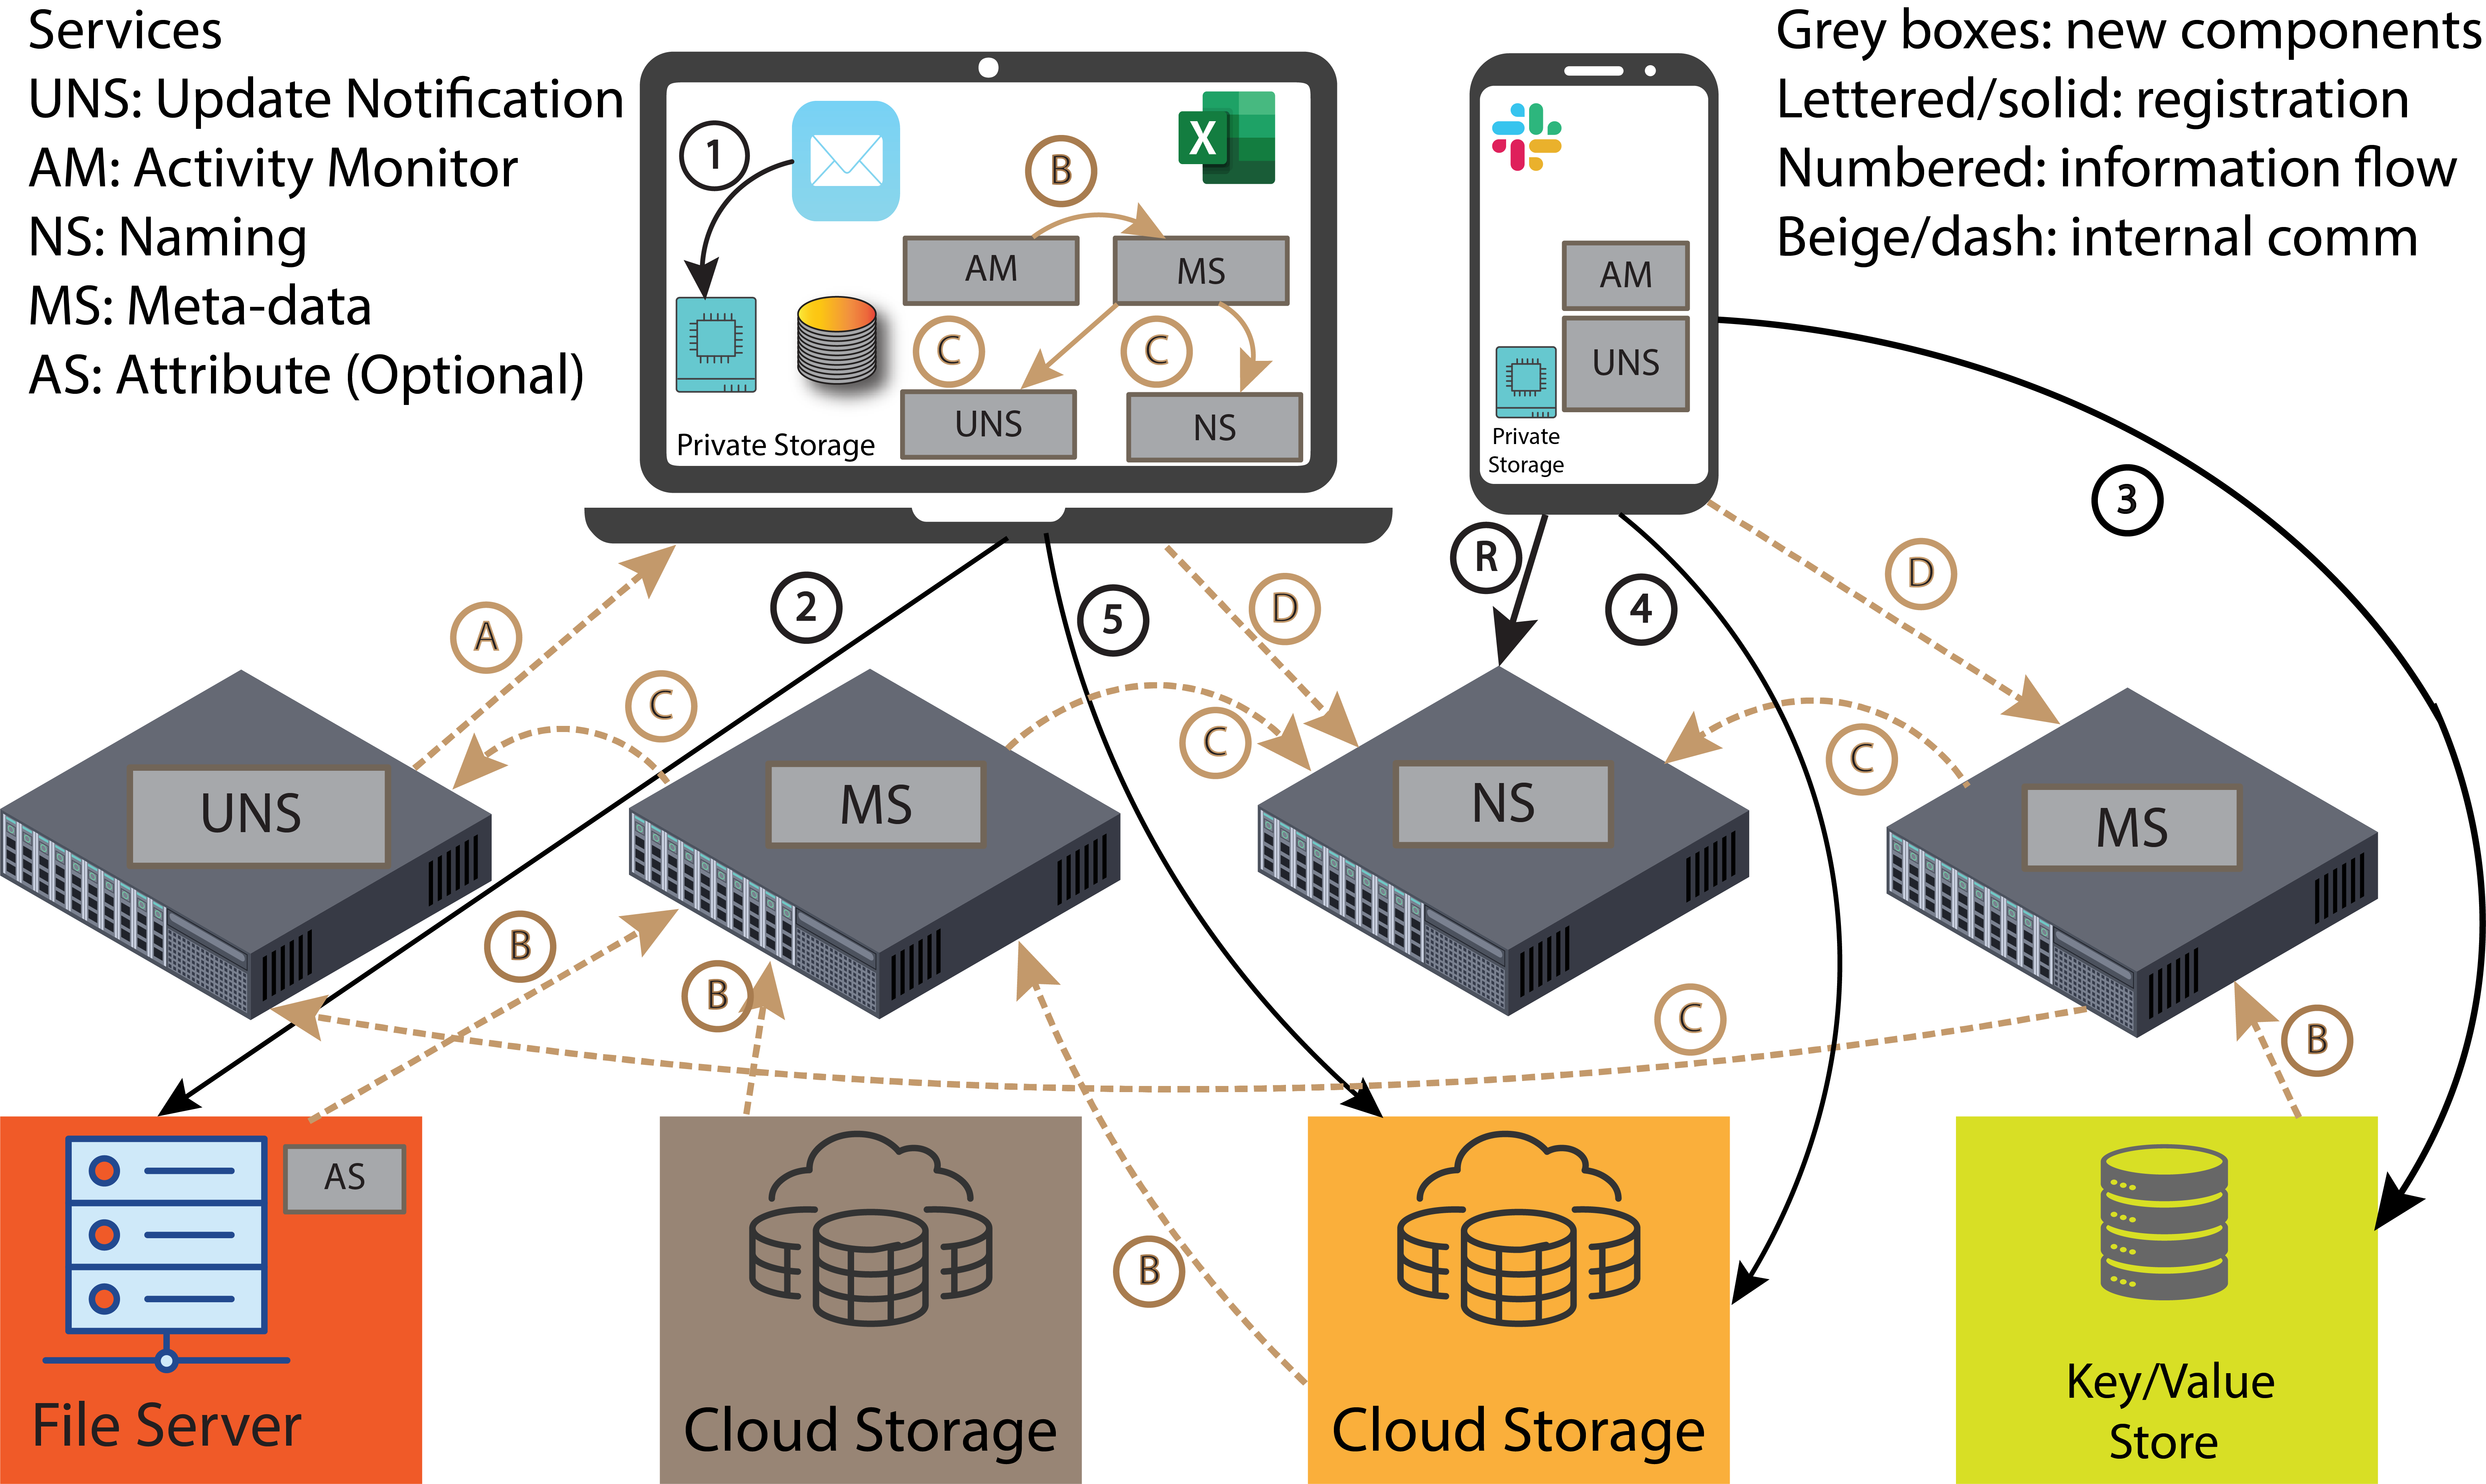
\includegraphics[width=0.95\textwidth]{reference/hotstorage21/figures/Naming5-legend.png}
    \caption{\system Architecture (\autoref{ch:architecture:sec:proposed-architecture}).
        %Grey boxes indicate new components. AM=``Activity Monitor'', MS=``Meta-data Server'', UNS=``Update Notification Server'', NS=``Namespace Server''.
    }
    \label{fig:arch}
\end{figure}

\autoref{fig:arch} illustrates the \system architecture. \system allows for
different deployment scenarios. The five services can be run independently, they
can be co-located and bundled together to run on a local device, integrated into
an OS, or available as web-based services.

In the balance of this section, parenthesized numbers and letters refer to the arrows
in Figure \ref{fig:arch}. There are five main components:

\begin{enumerate}

    \item \textbf{Metadata servers (MS)} are responsible for storing attributes
          and provide a superset of capabilities found in existing metadata
          services~\cite{federatedMetaData,smartstore}. Users can register a
          Metadata Server with
          activity monitors or attribute services, which allows the Metadata Server to receive
          updated attributes from storage objects and activities (B). Thus, there can
          be multiple sources of attributes including the user itself. Metadata
          servers may retain the full or partial history of attribute updates or
          maintain only the most recent value.

    \item \textbf{Namespace servers (NS)} connect to one or more Metadata Server and use the metadata to provide users with a
          personalized namespace that allows both manual organization (i.e., a
          hierarchical namespace) and rich search capabilities.  The benefit of
          supporting a hierarchical namespace is that it provides a path for
          backwards compatibility as well as a mechanism for enabling virtual
          directories~\cite{gifford1991semantic} to enable existing applications
          to benefit from the enhanced capabilities of \system.  The benefit of
          rich search capabilities is that it enables us to build those virtual
          directories for use by the hierarchical components as well as propose
          and evaluate alternative data exploration tools.
          Users can register with a Namespace Server (R) that uses one or more Metadata Servers to obtain relevant
          attributes from them (C). Additionally, users can be part of a corporate Namespace Server that
          allows sharing of their select metadata with other users via standard enterprise
          public-key cryptography.

    \item \textbf{Activity monitors (AM)} run on the user's devices. Their main function is to observe temporal relations,
          activity context, and relationships between objects on a user's device and
          transmit them to a Metadata Server (D).

    \item \textbf{Attribute services (AS)} extract attributes from storage objects and transmit them to an Metadata Server (B). An Attribute Service
          might be invoked on updates, run once or periodically. For example, a file
          system Attribute Service would update the object's metadata with basic attributes such as size
          or modification time. There can be many Attribute Services that extract more ``interesting''
          attributes, e.g., image recognition, similarity, or other classifiers.

    \item \textbf{Update notification server (UNS)} provides notification mechanisms. Users can register interest in changes of
          attributes or underlying storage and will receive a message on change events (A)
          to which they have access.

\end{enumerate}

In \autoref{fig:single-system} I show a simplified image depicting how this
might work on a single computer system, with data collection from a variety of sources on
the local computer, including resources that are both local to the system and
remote resources accessible and in use on the computer.  Information is
ingested by the local \system components and then presented to applications via
a query interface; one likely use of this query interface would be using it to
form ``virtual directories'' that allow legacy application interactions with the
namespace. Unlike \autoref{fig:arch} this diagram omits details of the internal
structure and instead explains one way in which it could fit into the local
device's environment.

\begin{figure}
    \centering
    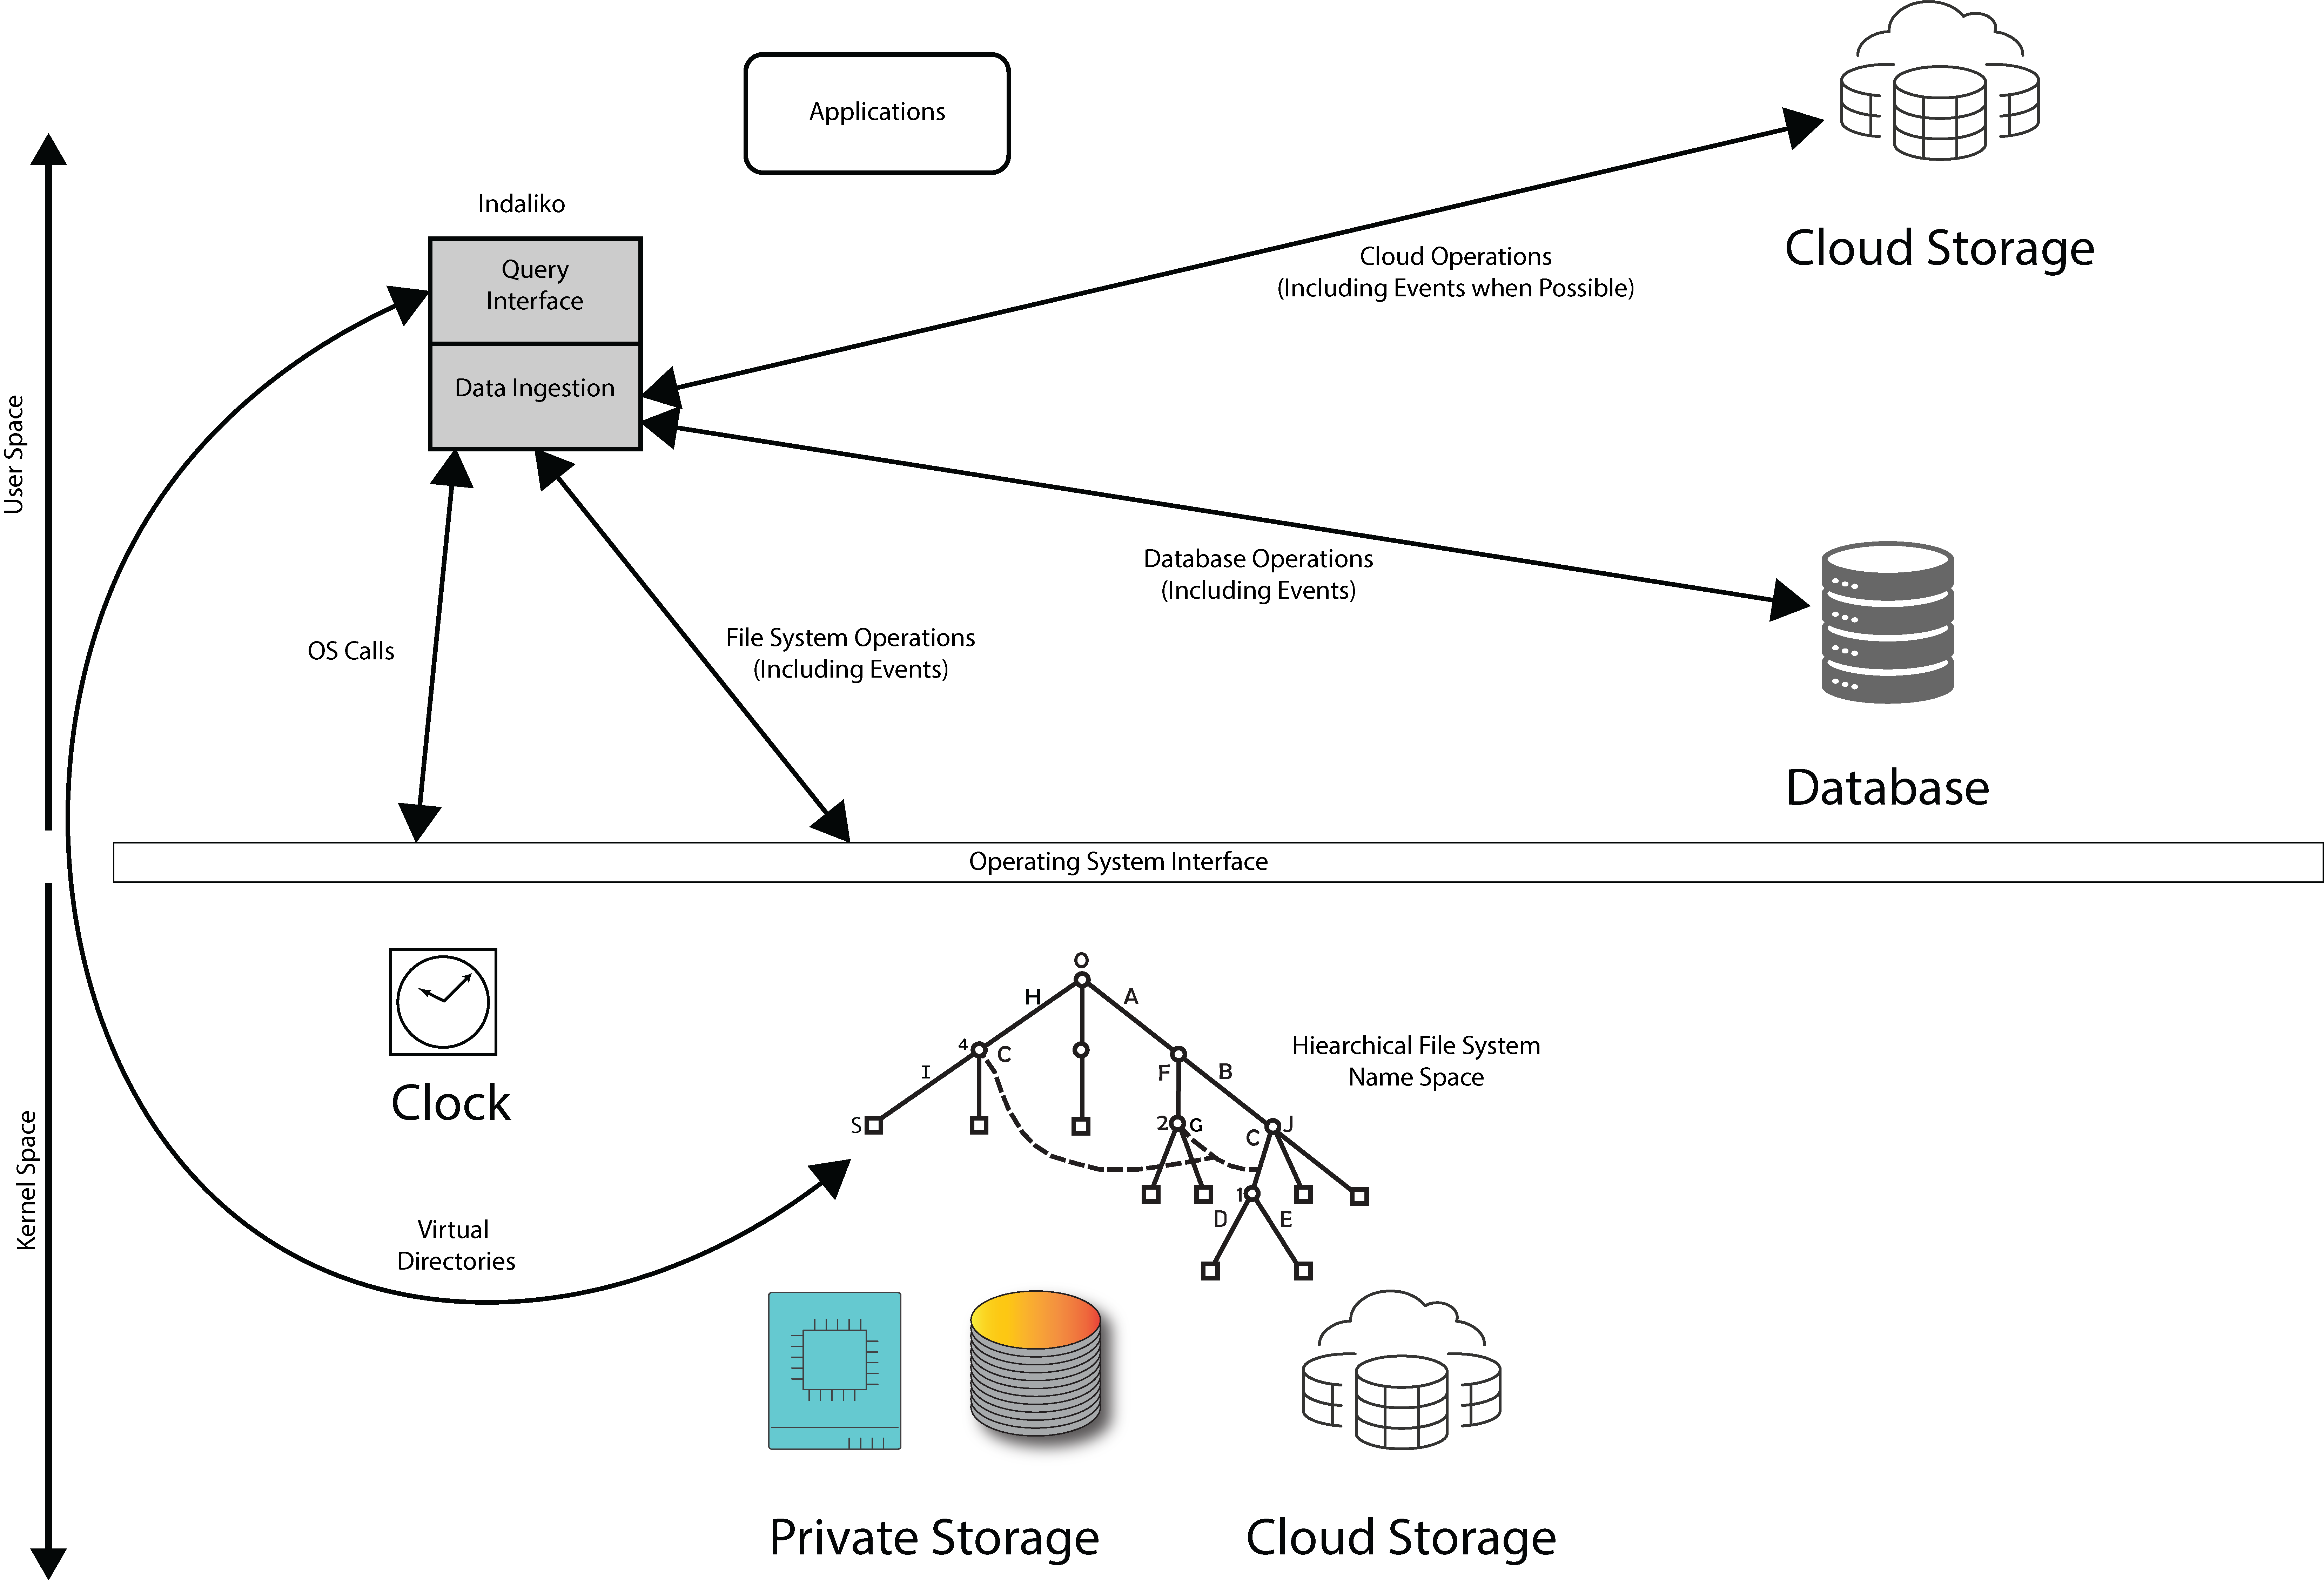
\includegraphics[width=0.95\textwidth]{figures/indaleko-arch.png}
    \caption{Single computer components for \system.}
    \label{fig:single-system}
\end{figure}


\section{\system Working Example}
\label{ch:architecture:sec:working-example}

To make the \system architecture concrete, I revisit our use-cases from \autoref{table:usecases}
and walk through the cases to illustrate how \system supports the various actions and events.

\subsection{Storing the e-mail attachment}

\persa's act of saving the CSV file that \persc sent in email corresponds to the
creation of a new object on the cloud storage silo, i.e., the file system (4). The
file server is \system-aware, so the Attribute Service co-located with it extracts attributes
from the document and forwards them to the Metadata Server (B).

The Activity Monitor on \persa's laptop detects that the CSV file came via company email from
\persc. It then captures the activity context identifying the relationship
between the e-mail and the CSV file and transmits it as additional metadata
about the CSV file to the Metadata Server (that already contains metadata extracted by the
Attribute Service). Moreover, because there is a company-wide namespace service, \system
establishes that the e-mail attachment, the CSV in the file server, and the one
on \persc's laptop (from which the file was sent) are exact copies of each
other.

Many applications already record some form of activity context, e.g., chat
history, browsing history. Such histories provide a rich source of additional
metadata. Other activity context, specifically the relationship between objects,
such as the fact that a particular file was saved to a local storage device from
an email message, requires more pervasive monitoring as found in, e.g., whole
provenance capture systems~\cite{camflow}. \system is agnostic about the precise
data that comprises activity context, but allows for storing and accessing
activity context as metadata.

\subsection{Creating the Excel file}

\persa opens the comma separated value (CSV) file using Excel and stores it as a spread sheet.
This creates a new object. The Activity Monitor detects that the newly created spreadsheet is
a conversion from the CSV file, either via a notification from \system-aware
Excel or by monitoring the system calls executed on the local system. \persa
proceeds to modify the data by filtering it in Excel and saving the changes. The
Activity Monitor records this event and updates the meta-data of the spreadsheet to record the
derivation-relationship. Ideally a \system-aware version of Excel specifies to
the Activity Monitor the exact type of the relationship (in this case a derivation); otherwise
the Activity Monitor informs the Metadata Server about an unspecified data relationship by observing the
opening of a CSV file and a subsequent creation of the Excel file.

\persa proceeds to upload the new Excel file on Slack, which triggers the
creation of a new storage object as Slack creates a local copy, the addition of
new metadata to Metadata Server via the AS, and the addition of a \emph{copy} data relationship
between the original Excel file and the Slack’s copy. The Activity Monitor notices (by
monitoring Slack chat) that the file was shared with user \persc and promptly
notifies the Metadata Server, which adds this detail to its metadata.

Once \persa is done, its local Metadata Server has been updated with three new objects: the
CSV file, the corresponding Excel file, and Slack’s copy of the Excel file.
There is a data relationship linking all three and metadata informing us
that the original CSV came from \persc and that the final Excel file was also
shared with that same person. If \persa wanted to remember what happened to
the data from the original CSV from \persc, they could query their local
personal Namespace Server, which would track down this history by querying the Metadata Server metadata.

\subsection{Sharing the spreadsheet}

\persc receives the Excel file from \persa via Slack on their phone, a
sequence of metadata events similar to those described earlier takes place,
except the phone does not run a local Namespace Server or Metadata Server. \persc now uploads the file to
the company's cloud drive (4). The Metadata Server (by way of the Attribute Service) reflects the creation of a
new object and records its remote location. The use of a company-wide namespace
and metadata service enables \system to record that the file in the cloud drive
is, in fact, a copy of the one received via Slack.  Further, \persc informs
their personal Namespace Server that they wish to notify \persa about all updates to the file
on the cloud drive. Thus, whenever an Attribute Service sends updated attributes to the Metadata Server,
\persc receives a notification.

The sharing relationship between the personal Namespace Server of \persa and \persc, and the
exchange of the relevant cryptographic credentials, would have been set up
earlier.

\subsection{Data origin and delete requests}

When the compliance officer asks about the origin of the data, \persc can query
the corporate Namespace Server to obtain the complete history of the report. This includes the
spreadsheet from which the report was derived and the e-mail or Slack messages
that transmitted the files.

The corporate Namespace Server was configured to be aware of the locations of the
collaborating users' personal Namespace Server. Moreover, because of the activity contexts
captured by the Activity Monitor, \system is able to identify documents that were created
during any activity involving the customer whose data must be deleted. Starting
from these documents, and by using the relationship of documents, \persb was
able to find all relevant objects and delete them, including the e-mail and
Slack messages.

\persa would have configured their personal Namespace Server to allow sharing of the metadata
associated with \persc with their corporate Namespace Server, and \persc would configure their
personal Namespace Server similarly. As a result, when \persc issues to the corporate Namespace Server a
query asking to trace the origins of the data in the final report, the corporate
Namespace Server is able to return all the history tracing back to the original CSV file.

Note that unlike existing systems, \system is able to efficiently find related
objects across storage silos. Operating systems already provide users with
indexing services to accelerate search of local files. This search can be made
cross-silo by mounting and enabling indexing on network shares (e.g., Windows
Desktop Search), or by interfacing with specific applications such as e-mail
(e.g., MacOS Spotlight, or Android search). The problems with indexing a
large remote storage repository are resource limitations such as bandwidth. In contrast,
\system addresses these limitations by delegating indexing and storage to one or
more services.

Namespace Servers are responsible for providing efficient search functionality.
\system uses Attribute Services to keep attributes up to date with object
modifications. Lastly, \system
supports coordinated search among one or more local and remote Namespace Server, allowing, for
example, a user to search across both their local Namespace Server as well as their employer's
Namespace Server.

\endinput

\section{Research Questions}
\label{ch:arhitecture:sec:research-questions}

Given the broad research questions that I provided in
\autoref{ch:research-questions}, it is important to also explain how my proposed
architecture is motivated to answer those questions.

\begin{comment}
% Moved to the original RQs
The questions themselves that are core to my proposed thesis work revolve around
exploring and broadening the earlier idea of an \emph{activity context}.
However, activity context by itself does not replace the other prior work that
has added semantic understanding around files, e.g., semantic file systems,
formal concept analysis, tag file systems, graph file systems, etc. Thus, my
proposed system includes support for this prior work but extends it by
augmenting previous mechanisms with this additional rich usage information that
I call ``activity context.''
\end{comment}


\subsection{Events}

Research questions \ref{rq:define-ac} and \ref{rq:capture-ac} relate to
identifying and capturing the specific events on a user's device that yield the
insights necessary to answer research question \ref{rq:leverage-ac}.  While
prior work~\cite{provsearch,vianna2014a} has proposed partial answers to these
questions, I will do the additional work necessary to address my own thesis by
looking broadly at combining this prior work as well as considering adding
additional contemporaneous events that seem likely to be beneficial.

My architecture is sufficiently general that it envisions having a stream of
event information that can then be used to better understand the context in
which digital objects are created and used.  While some of this has been
suggested previously under the guise of ``personal digital
traces''~\cite{vianna2019searching}, it is important to provide a simple
mechanism for extending the data collection and providing it in a uniform
fashion that can be used to further explore development of new tools. While I
have suggested a couple of potentially novel ideas, such as identifying the
music that was playing, I expect there will be other information that can be
collected.  For example, eye tracking information could be used to determine
more about the relationship between various elements.  Other sensory information
could be incorporated: the smells of cooking, the sounds of others within the
user's environment, their conversations, etc.  These become an extension of the
personal digital traces into a \emph{personal environmental trace}.

A key challenge here is to find a common language for describing these events;
while there is some effort at doing so in the personal digital traces work, it
is likely that I will need to extend that model to accommodate the various data
sources I have described (see \autoref{table:useful-information}.)


I envision a key aspect of this work will be to consider the personal digital
traces work and design an application programming interface (API) that I will
use for collecting the event traces into my implementations against this
interface.

Providing support for collecting, storing, and making this event information
accessible is a key element of the work that I propose providing in support of
my thesis.

\begin{comment}
\subsection{Improved Access}

Research question \ref{rq:improve} focuses on verifying that \emph{activity
    context} yields better outcomes.  Mentally, I consider this question to be
determining if the \emph{finding} outcome for digital objects is improved: does
it take less time to find things, does the user find things they had forgotten
about but wanted to find, does it improve their satisfaction, and does it
decrease them reaching the point of giving up their search.

While I do not propose answering this research question as part of my work for
this thesis, I do note that my proposed architecture provides the systems level
framework to better explore this space by enabling a simple model for collecting
activity context data as well as accessing that information.  Thus, by making
the collection and dissemination easier, it will be simpler for other
researchers to explore the effectiveness of activity context.
\end{comment}


\subsection{Compatibility}

I need to evaluate how existing applications can take advantage of the richer
meta-data capabilities I will make available in order to fully answer research
question \ref{rq:leverage-ac}.
Prior work has suggested ``virtual
directories'' as one way to achieve this and that may be sufficient, however
there are other models that have also been suggested, including graph name
spaces~\cite{gfs}, alternative browsers~\cite{9502515,collins2010escaping},
as well as hybrid models in which automated classifiers are either explicitly or
implicitly determined~\cite{10.1145/3209900.3209911}.

\subsection{Meta-Data Query}
\label{ch:architecture:sec:rq:subsec:meta-data-query}

Research question \ref{rq:meta-data-query} relates to asking how we provide
activity context to enable others to exploit it in building new tools and
exploring related research questions for refining and developing further tools.
There is a strong body of prior work regarding meta-data queries of both static
and dynamic
sources~\cite{Strong,revol2011universal,smartstore,pindex,federatedMetaData,huo2016mbfs,Suguna2015,Parker-Wood2014,watson2017exploring,leung2009magellan,leung2009spyglass,niazi2017hopsfs,van2011efficient}.

My architecture proposes using a meta-data service for storing and accessing
activity context information.  I did this precisely to allow support for a
flexible and fast query mechanism and thus the architecture does provide the
tools necessary to answer this research question as part of the work that I
propose in supporting my thesis.

\subsection{Privacy}

Research question \ref{rq:privacy} raises the issue around protecting sensitive
personal information.  My architecture permits a secure implementation of collecting detailed personal
information by giving the user the ability to restrict the sharing of that
information.  The architectural model envisions a more generalized framework in
which service providers can use existing or new authentication and encryption
mechanisms for supporting both ``Context as a Service'' models for service
providers, as well as enabling selective sharing of sensitive information with
other users.  While I do not propose exploring this research question broadly,
the architecture provided is sufficient to answer it narrowly.  Such a narrow
definition does not preclude future research into a more permissive model that
remains consistent with the proposed architecture.


